%% S8: no closed S-term p is convertible with E[p] for a plain context E of depth at most 2.
%% DRAFT 2026-11-24 (skinock).  Neutral amsart shell, as S1--S7.
%% Sources: ~/Code/ski/notes/NCFP-proof.md (sections 2--3, 9.1, 11.1, 12.2, 13.1, 15.1--15.4, 16.1) and the
%%          NCFP section of ~/Code/ski/notes/A1-lock1-S3.md (Lemma L, Theorem 2), with their Wizard reviews.
%% Paper-to-Lean map (lean-ski v1.16.0, modules Ski/Ncfp*.lean, namespace Ncfp; all in #audit_clean):
%%   thm:main ....... ncfp_depth2 (Ski/NcfpPlain.lean; PlainD, plain1_cases)
%%   thm:two ........ right_combs, right_combs_seq, right_combs_conv
%%   lem:invariant .. hnf1_conv, hnf2_conv; S6: Conv
%%   lem:distinct ... Desc.irrefl, desc_finite, finite_descent (from HeadRec.no_ground_loop)
%%   lem:frames ..... (a) lemma_L, lemma_L', hnf1_literal; (b) last_item_step, fact_LI; (c) lemma_P, lemma_P3
%%   lem:td ......... lemma_TD            lem:ss ......... lemma_SS, lemma_SS_sz, cor_SS1
%%   lem:last ....... (a) lemma_LL; (b) lemma_SR, cor_LL1
%%   lem:dstar ...... lemma_Dstar, dstar_frames
%%   thm:xplus ...... thm_Xplus (XplusSet; xp_cases, xp_pred, xp_block, xp_small)
%%   cor:x1 ......... cor_X1 (sets, all three kinds of second entry); ncfp_X1 (contexts; second entry
%%                    S E' or S n E' only -- the kind S E' n is NOT in the Lean context statement)
%%   lem:eq ......... no single declaration; built inside ncfp_X1 (simpB_hnf), ncfp_holes, ncfp_scheme
%%                    (typed_of_reps) and the equations no_S_*; (NN) is typed_nn, not_normalizing
%%   lem:leaf ....... (a) lemma_ZA_two, lemma_ZA_one; (b) lemma_NH, lemma_ZI_i, lemma_ZI_ii
%%   lem:survive .... inside theta_chain / pr_members (step 3 of the note's Theorem Theta)
%%   lem:prim ....... lemma_PR, pr_members, pr_one, leafless_chain
%%   thm:leafless ... thm_L, thm_L_bounded        cor:holes ...... ncfp_holes
%%   Section 5 ...... thm_N3 (no_S_Snp_p), thm_N4 (no_S_Spn_p), thm_T3a..thm_T3d (no_S_Spp_Snp,
%%                    no_S_Spp_Spn, no_S_Snp_Spp, no_S_Spn_Spp); the Lean proofs take other routes
%%                    (right_combs' for N3, N4; three_X = thm_X for T3a--d)
%%   cor:fpc ........ no_fpc, no_fixed_point_combinator, ncfp_S
%% Terms applied to arguments (bmove, lemma_A, lemma_T, teeth_unbounded, cor_B1, cor_B1' and NcfpC of
%% v1.17.0) are the subject of S9, which this paper cites in the closing only.
%% TODO: restructured 2026-11-24 (the section on terms without an hnf moved to S9): Grammarian on
%% the prose, then Wizard on this text.
\documentclass[11pt]{amsart}
\usepackage[T1]{fontenc}
\usepackage{lmodern}
\usepackage{amsmath,amssymb,amsthm}
\usepackage{graphicx}
\usepackage[numbers,sort]{natbib}
\usepackage[hidelinks]{hyperref}
\usepackage{bm}

\newtheorem{theorem}{Theorem}
\newtheorem{lemma}[theorem]{Lemma}
\newtheorem{corollary}[theorem]{Corollary}
\newtheorem{conjecture}[theorem]{Conjecture}

\newcommand{\Ter}{\mathcal S}
\newcommand{\red}{\twoheadrightarrow}
\newcommand{\hred}{\twoheadrightarrow_h}
\newcommand{\conv}{=_\beta}
\newcommand{\sz}[1]{\lvert#1\rvert}
\newcommand{\fr}[1]{[#1]}

\title[No Conversion Fixed Points in Plain Contexts]{No Conversion Fixed Points in Plain Contexts of the Combinator $\bm{S}$}
\author{Claude Opus \& Fable with N.\ E.\ Davis}
\address{ZeroAttest, Champaign, Illinois, USA}
\email{NDavis@ZeroAttest.com}
\urladdr{https://orcid.org/0000-0002-1131-8319}
\date{\today}

\begin{document}
\begin{abstract}
We show that no closed term $p$ of the combinator $S$ is convertible with $E[p]$ when $E\ne[\,]$
is a plain context of depth at most two with a hole. A context is plain if it is built from holes
and closed normalizing terms by $E'\mapsto S\,E'$ and $E',E''\mapsto S\,E'\,E''$. The proof rests
on three theorems. An infinite right comb has teeth of unbounded size. No nonempty set of terms
has these two properties: every member has a head normal form whose items lie in the set or are of
bounded size, at least one of them in the set; and the last head step of a member duplicates a
large item in two simple ways only. No nonempty set meets only finitely many conversion classes if
every member has a head normal form with at least one item and all its items in the set; this
settles every plain context without closed parts. The case $E=S\,[\,]$ gives Statman's theorem that
$S$ defines no fixed-point combinator.
\end{abstract}

\keywords{combinatory logic, combinator $S$, head reduction, fixed points, convertibility}
\maketitle

\section{Introduction}

$\Ter$ is the set of closed terms built from $S$ by application, with $S\,x\,y\,z\to x\,z\,(y\,z)$ at
any position; $\to^+$ and $\red$ are the transitive and the reflexive--transitive closure of $\to$,
and $\conv$ is convertibility. The
\emph{size} $\sz t$ is the number of occurrences of $S$ in $t$; a step never lowers it, since $z$
contains an $S$. A term is \emph{normalizing} if it reduces to a normal form $n$; every term
convertible with it then reduces to $n$, by Church--Rosser, and has size at most $\sz n$. A
\emph{ground loop} is a reduction $t\to^+u$ with $t$ a subterm of $u$; there is none in
$\Ter$~\citep{waldmann-ic,s7}.

Every $t\in\Ter$ is $S\,u_1\cdots u_m$ for a unique $m\ge0$. We write this \emph{frame} as
$\fr{u_1,\dots,u_m}$; the $u_i$ are its \emph{items}, and $t$ is a \emph{head normal form} (hnf)
if and only if $m\le2$. If $m\ge3$, the \emph{head step} leads to $u_1\,u_3\,(u_2\,u_3)\,u_4\cdots u_m$, whose
items are those of $u_1$ followed by $u_3,\ u_2\,u_3,\ u_4,\dots,u_m$. The successive head steps
from $t$ form its \emph{head run}, and $\hred$ is the reflexive--transitive closure of the head
step. If the head run of $t$ reaches an hnf $h$, then $t$ \emph{has the hnf} $h$, and $t$ is
\emph{literal} if $t=h$. If $t\ne h$, the frame just before $h$ is the \emph{last frame} of $t$.

A \emph{context} $E$ is a term with holes $[\,]$; $E[p]$ fills every hole with $p$, and $E$ is
\emph{closed} if it has no hole. The \emph{plain} contexts are the hole, the normalizing terms of
$\Ter$, and $S\,E'$ and $S\,E'\,E''$ for plain $E'$, $E''$. A closed plain context is a normalizing
term. The \emph{depth} of a plain context is $0$ if it is the hole or closed; otherwise it is one
more than the depth of $E'$ for $S\,E'$, and one more than the larger of the depths of $E'$, $E''$
for $S\,E'\,E''$.

\begin{theorem}\label{thm:main}
Let $E\ne[\,]$ be a plain context of depth at most $2$ with at least one hole. Then no $p\in\Ter$
satisfies $p\conv E[p]$.
\end{theorem}

\noindent With $p$ for the hole and $n$ for a closed part, these are the contexts $S\,X$ and
$S\,X\,Y$ with $X,Y$ among $p$, $n$, $S\,p$, $S\,p\,p$, $S\,n\,p$, $S\,p\,n$, not both closed: $40$ shapes.
Corollary~\ref{cor:holes} covers the $12$ shapes without a closed part, and every plain context
without closed parts. Corollary~\ref{cor:x1} covers $22$ of the other $28$, and also plain
contexts of any depth whose closed parts sit at suitable places. Section~\ref{sec:main} treats the
remaining six. Figure~\ref{fig:trees} shows three of the shapes. Every proof rests on Theorem~\ref{thm:two}, and through
it on the absence of ground loops.

\begin{theorem}[right combs]\label{thm:two}
There are no $M$ and sequence $q_0,q_1,\dots$ in $\Ter$ such that every $q_n$ has the hnf
$S\,q_{n+1}$, or $S\,a_n\,q_{n+1}$ with $\sz{a_n}\le M$.
\end{theorem}

\noindent A \emph{right comb} is a sequence $q_0,q_1,\dots$ in which every $q_n$ has the hnf
$S\,q_{n+1}$ or $S\,a_n\,q_{n+1}$; the $a_n$ are its \emph{teeth}. So no right comb has teeth of
bounded size.

\begin{figure}[t]
\centering
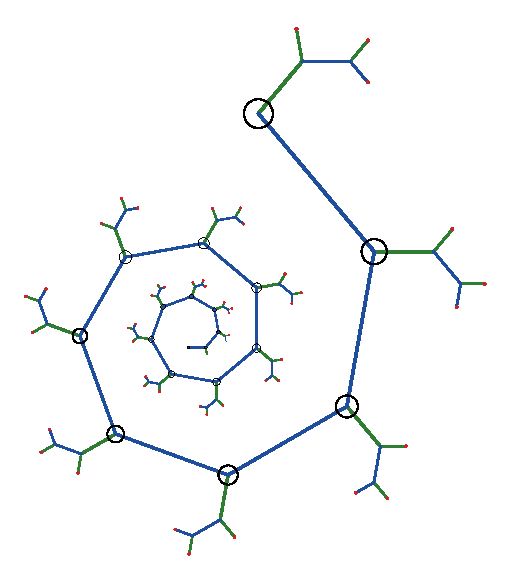
\includegraphics[height=0.27\textwidth]{fig/02-teeth.pdf}\hfill
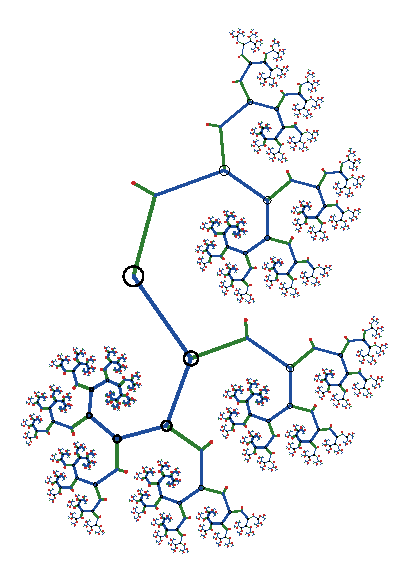
\includegraphics[height=0.27\textwidth]{fig/05-theta.pdf}\hfill
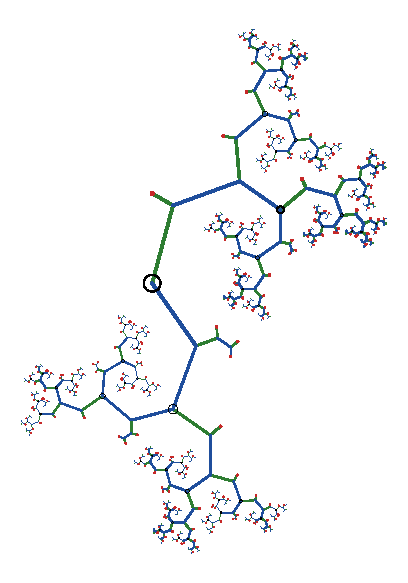
\includegraphics[height=0.27\textwidth]{fig/09-threehole.pdf}
\caption{The solution $T_E$ of $T=E[T]$ for three contexts $E$, with $n=S\,S$: $S\,n\,[\,]$ to
depth $18$, and $S\,[\,]\,[\,]$ and $S\,(S\,[\,]\,[\,])\,(S\,n\,[\,])$ to depth $14$. Function edges
are green, argument edges blue, leaves $S$ red; a ring marks a node at which $T_E$ recurs. A term
$p\conv E[p]$ would have $T_E$ as its infinitary normal form~\citep{s3}. By
Corollaries~\ref{cor:x1} and~\ref{cor:holes} and Theorem~\ref{thm:main}, respectively, no such $p$ exists.}
\label{fig:trees}
\end{figure}

\section{Head runs}\label{sec:runs}

The frames on the head run of a term $f$ without an hnf have at least three items, so the head run
of $f\,w$ is that of $f$ with $w$ appended, and $f\,w$ has no hnf. The next lemma
is~\citep[Lemma~4]{s6}, applied to the model of terms modulo $\conv$: convertible terms have
hnfs with equally many items, convertible in order.

\begin{lemma}[\citep{s6}]\label{lem:invariant}
Let $t\conv t'$. If $t$ has the hnf $\fr{u_1,\dots,u_m}$, then $t'$ has an hnf $\fr{u'_1,\dots,u'_m}$
with $u_i\conv u'_i$ for all $i$.
\end{lemma}

\begin{lemma}\label{lem:distinct}
Let $t_0,t_1,\dots$ in $\Ter$ be such that each $t_j$ reduces to a term of which $t_{j+1}$ is a
proper subterm; for instance, $t_{j+1}$ is an item of the hnf of $t_j$. Then the $t_j$ are pairwise
distinct, and for every $M$ only finitely many of them have size at most $M$.
\end{lemma}

\begin{proof}
Reduction acts inside subterms, so for $i<j$, $t_i$ reduces to a term $u$ of which $t_j$ is a
proper subterm. If $t_i=t_j$, then $u\ne t_i$, and $t_i\to^+u$ is a ground loop, and no such reduction
exists~\citep{waldmann-ic,s7}. There are finitely many terms of size at most $M$.
\end{proof}

A \emph{comb context} is $C=c_k\,(\cdots(c_1\,[\,])\cdots)$ with $c_i\in\Ter$ and $k\ge0$.

\begin{lemma}\label{lem:frames}
Let $F\to F'$ be a head step, where $F=\fr{u_1,\dots,u_m}$.

\textup{(a)} $F'$ has $m-1$ items more than $u_1$, so at least two. Hence a term with the hnf $S$ or
  $\fr{a}$ is literal, and a term that is not literal and has an hnf has a last frame $\fr{S,y,z}$
  and the hnf $\fr{z,y\,z}$.

\textup{(b)} If $m\ge4$, then $F'$ has the last item of $F$, and the step is a head step of
  $\fr{u_1,\dots,u_{m-1}}$ with $u_m$ appended. If $m=3$, the last item of $F'$ is $u_2\,u_3$. Hence,
  on the head run of a term with last item $u$, every frame has a last item $C[u]$ with $C$ a comb
  context, and $C=[\,]$ if and only if no earlier frame has exactly three items.

\textup{(c)} If $F'=\fr{x,p,q}$, then $F=\fr{S\,x,b,p}$ with $q=b\,p$, or $F=\fr{S,b,x,q}$ with $p=b\,x$.
\end{lemma}

\begin{proof}
The items of $F'$ are those of $u_1$, then $u_3,\ u_2\,u_3,\ u_4,\dots,u_m$. This gives (a)
and (b); in (a), exactly two items occur only when $m=3$ and $u_1=S$. In (c), either $u_1=S\,x$ and $m=3$, with
$(u_3,u_2\,u_3)=(p,q)$, or $u_1=S$ and $m=4$, with $(u_3,u_2\,u_3,u_4)=(x,p,q)$.
\end{proof}

\begin{lemma}\label{lem:td}
Let $t$ have at least three items and an hnf, with last frame $\fr{S,y,z}$. Then either
\textup{(A)} no earlier frame has exactly three items, and then $t=t^-\,z$ with
$t^-\hred\fr{S,y}$; or \textup{(B)} the last earlier frame with exactly three items is
$\fr{x,p,q}$, and then $x\ne S$, $z=p\,q$ and $x\,q\hred\fr{S,y}$.
\end{lemma}

\begin{proof}
We use Lemma~\ref{lem:frames}(b). In (A) all frames before the last have at least four items, so
the steps are head steps of $t^-$ with $z$ appended. In (B) the step from $\fr{x,p,q}$ leads to
$x\,q\,(p\,q)$; here $x\ne S$, since $\fr{S,p,q}$ steps to an hnf and would be the last frame.
The later frames before the last have at least four items, so the steps are head steps of $x\,q$
with $p\,q$ appended.
\end{proof}

\begin{lemma}\label{lem:ss}
If $\varphi$ has $k\ge2$ items and $\varphi\hred\fr{S,y}$, then
$\varphi=\fr{S,c,S,\dots,S}$ and $y=c\,S\cdots S$, each with $k-2$ trailing $S$; so
$\sz\varphi=\sz y+2$. Hence there is no infinite sequence $y_0,y_1,\dots$ with
$y_i\hred\fr{S,y_{i+1}}$ for all~$i$.
\end{lemma}

\begin{proof}
By induction on $k$. If $k=2$, then $\varphi$ is an hnf and $\varphi=\fr{S,y}$. Let $k\ge3$ and
apply Lemma~\ref{lem:td} to $\varphi$: its hnf $\fr{S,y}$ is $\fr{z,y'\,z}$, so $z=S$ and $y=y'\,S$.
Since $z$ is not an application, (A) holds: $\varphi=\varphi^-\,S$ and
$\varphi^-\hred\fr{S,y'}$, and the induction hypothesis applies to $\varphi^-$. In a sequence as
stated, every $y_i$ has at least two items, since $S$ and $\fr{a}$ are their own hnfs, and
$\sz{y_{i+1}}=\sz{y_i}-2$.
\end{proof}

\begin{lemma}\label{lem:last}
Let $w=g\,u$ have a two-item hnf $\fr{h_1,h_2}$. Then $\sz u\le\sz{h_2}$. If $u\ne S$ and
$\sz{h_1}<\sz u$, then $w$ is literal: $g=S\,h_1$ and $h_2=u$.
\end{lemma}

\begin{proof}
A literal $w$ is $\fr{h_1,u}$. Let $w$ be not literal; then $\sz{h_2}>1$. Let $u\ne S$ and apply
Lemma~\ref{lem:td}. In case (A), $h_1=u$. In case (B), $h_1=p\,q$, and $q$ contains $u$ by
Lemma~\ref{lem:frames}(b). In both cases $\sz{h_2}>\sz{h_1}\ge\sz u$.
\end{proof}

\begin{lemma}\label{lem:dstar}
Let $w=g\,u$ have at least three items and an hnf, and let $\sz u\ge3$. Then $g$ has a two-item hnf
$\fr{b,a}$, and the hnf of $w$ is \textup{(A)} $\fr{u,a\,u}$ if $b=S$; \textup{(B)}
$\fr{a\,u,u\,(a\,u)}$ if $b=S\,S$; \textup{(C)} $\fr{p\,q,q\,(p\,q)}$ otherwise, where $p=C[u]$ for a
comb context $C$ and $q=g'\,p$ for some $g'$.
\end{lemma}

\begin{proof}
(1) \emph{If $f\,m$ has at least three items and an hnf, then $f$ has a two-item hnf $\fr{f',g'}$,
and the first frame with three items on the head run of $f\,m$ is $\fr{f',g',m}$.} By
Lemma~\ref{lem:frames}(b) the run of $f\,m$ follows that of $f$, with $m$ appended, as long as the
frames of $f$ have at least three items. The run of $f\,m$ is finite, so $f$ reaches a first frame
with at most two items; it has two, by Lemma~\ref{lem:frames}(a) or because it is $f$ itself.

(2) By (1), $w\hred\fr{b,a,u}$. If $b=S$, the next frame is the hnf $\fr{u,a\,u}$. If $b=S\,S$, the
next frames are $\fr{S,u,a\,u}$ and the hnf $\fr{a\,u,u\,(a\,u)}$.

(3) Let $b\notin\{S,S\,S\}$. A three-item frame $\fr{f,g,m}$ with $f\ne S$ steps to
$f\,m\,(g\,m)$, so by (1) the next three-item frame is $\fr{f',g',g\,m}$, where $\fr{f',g'}$ is the
hnf of $f\,m$; a three-item frame $\fr{S,g,m}$ is the last frame. So the three-item frames from
$\fr{b,a,u}$ on are $G_i=\fr{f_i,g_i,m_i}$, $0\le i\le r$, with $m_0=u$, $m_{i+1}=g_i\,m_i$,
$\fr{f_{i+1},g_{i+1}}$ the hnf of $f_i\,m_i$, and $f_r=S$; here $r\ge1$. Every $m_i$ is $C_i[u]$ for a
comb context $C_i$, so $\sz{m_i}\ge3$. The hnf of $f_{r-1}\,m_{r-1}$ is $\fr{S,g_r}$, so by
Lemma~\ref{lem:last}, $f_{r-1}=S\,S$ and $g_r=m_{r-1}$. Put $p=g_{r-1}$ and $q=m_{r-1}$: then
$G_{r-1}=\fr{S\,S,p,q}$, $G_r=\fr{S,q,p\,q}$, and the hnf of $w$ is $\fr{p\,q,q\,(p\,q)}$. Since
$f_0=b\ne S\,S$, we have $r\ge2$. The hnf of $f_{r-2}\,m_{r-2}$ is $\fr{S\,S,p}$, so by
Lemma~\ref{lem:last}, $p=m_{r-2}$, and $q=g_{r-2}\,p$.
\end{proof}

\begin{proof}[Proof of Theorem~\ref{thm:two}]
Suppose such $M$ and $q_0,q_1,\dots$ exist. If $q_n$ is literal, then $q_{n+1}$ is a proper subterm of $q_n$,
so infinitely many $q_n$ are not literal. For these, Lemma~\ref{lem:frames}(a) gives the last frame
$\fr{S,y_n,a_n}$ and $q_{n+1}=y_n\,a_n$. If $q_{n+1}$ is then literal, it is $\fr{a_n}$ or
$\fr{a_{n+1},a_n}$, so $q_{n+2}=a_n$ has size at most $M$; by Lemma~\ref{lem:distinct} this happens
finitely often. So a literal term follows a non-literal one finitely often, and from some $m$ on
no $q_n$ is literal. For $n\ge m$, the head run of
$q_{n+1}=y_n\,a_n$ ends in the last frame $\fr{S,y_{n+1},a_{n+1}}$, so $a_{n+1}=C_n[a_n]$ by
Lemma~\ref{lem:frames}(b). The sizes are bounded, so $C_n=[\,]$ from some $m'$ on; then case (A) of
Lemma~\ref{lem:td} holds for $q_{n+1}$, and $y_n\hred\fr{S,y_{n+1}}$ for all $n\ge m'$,
contradicting Lemma~\ref{lem:ss}.
\end{proof}

\section{Sets closed under items}\label{sec:sets}

\begin{theorem}\label{thm:xplus}
There are no $M\ge1$ and nonempty $Z\subseteq\Ter$ such that every $v\in Z$ has an hnf with one or
two items, each of them in $Z$ or of size at most $M$ and at least one of them in $Z$, and such
that, if $v$ is not literal and its last frame is $\fr{S,y,z}$, then $\sz z\le M$, or $y=S$, or
$y=S\,c$ with $\sz c\le M$.
\end{theorem}

\begin{proof}
Suppose such $M$ and $Z$ exist. Call a non-literal $v\in Z$, with hnf $\fr{z,y\,z}$, \emph{ordinary} if
$\sz z\le M$, and \emph{exceptional} otherwise; then $z\in Z$.

(E) \emph{Let $v$ be exceptional, with case (B) of Lemma~\ref{lem:td} and its frame $\fr{x,p,q}$.
Then $\sz x\le3$ and $\sz q\le M+1$.} Here $x\,q\hred\fr{S,y}$ and $x\ne S$, so $x\,q$ has $k\ge2$ items. By Lemma~\ref{lem:ss},
$x\,q=\fr{S,c_0,S,\dots,S}$ and $y=c_0\,S\cdots S$ with $k-2$ trailing $S$. Since $v$ is
exceptional, $y$ is $S$ or $S\,c$ with $\sz c\le M$. If $y=S$, then $k=2$ and $x\,q=S\,S\,S$. If $y=S\,c$, then $k=2$ and
$x\,q=S\,S\,(S\,c)$, or $k=3$ and $c_0=c=S$, $x\,q=S\,S\,S\,S$; for $k\ge4$, $S$ would be an
application. In each case $\sz x\le3$ and $\sz q\le M+1$.

Let $q_0\in Z$, and let $q_{j+1}$ be an item of the hnf of $q_j$ that lies in $Z$: any such item if
$q_j$ is literal, $y\,z$ if $q_j$ is ordinary and $y\,z\in Z$, and $z$ otherwise. By
Lemma~\ref{lem:distinct} we may assume $\sz{q_j}>M+3$ for all $j$. Then an ordinary $q_j$ has
$q_{j+1}=y\,z$ with $\sz z\le M$, and an exceptional $q_j$ in case (B) has $q_{j+1}=p\,q$ with
$\sz q\le M+1$; call these steps \emph{carrying}. After a carrying step, $q_{j+1}=f_{j+1}\,\ell_{j+1}$
with $\sz{\ell_{j+1}}\le M+1$. The other steps are \emph{shrinking}: $q_j$ is literal, or exceptional
in case (A), and $q_{j+1}$ is a proper subterm of $q_j$.

(1) \emph{If steps $j$ and $j+1$ are carrying, then $\ell_{j+2}=C[\ell_{j+1}]$ for a comb context
$C$, and if $C=[\,]$, then $f_{j+1}$ has the hnf $\fr{a,f_{j+2}}$ with $\sz a\le3$.} The term
$\ell_{j+2}$ is the last item of a frame on the head run of $q_{j+1}$: of the last frame
$\fr{S,y,z}$ if $q_{j+1}$ is ordinary, and of $\fr{x,p,q}$ otherwise. Apply
Lemma~\ref{lem:frames}(b). If $C=[\,]$, all earlier frames have at least four items, so the steps
to that frame are head steps of $f_{j+1}$, which reaches $\fr{S,y}$, resp.\ $\fr{x,p}$; and
$f_{j+2}$ is $y$, resp.\ $p$.

(2) \emph{There is no infinite run of carrying steps.} Along it the sizes $\sz{\ell_j}$ do not fall
and are at most $M+1$, so $C=[\,]$ from some point on, and the $f_j$ contradict
Theorem~\ref{thm:two}.

(3) \emph{If steps $n,\dots,n+r$ are carrying and step $n+r+1$ is shrinking, then $q_{n+r+2}$ is a
proper subterm of $q_n$.} Let $e=q_{n+r+1}=f\,\ell$ and $w=q_{n+r+2}$, so $\sz\ell\le M+1<\sz w$.
If $e$ were exceptional in case (A), or $e=S\,\ell$, then $w=\ell$. So $e=\fr{w,\ell}$. We show
$q_{n+r+1-i}=H_i\,\ell$ for $0\le i\le r+1$, where $H_i$ is an application whose argument contains
$w$; this holds for $i=0$ with $H_0=S\,w$. Let $i\le r$ and $j=n+r-i$. If $q_j$ is ordinary, its
last frame $\fr{S,y,z}$ has $y\,z=H_i\,\ell$; put $x=S$. Otherwise $q_j\hred\fr{x,p,q}$ with
$p\,q=H_i\,\ell$ and $\sz x\le3$, by (E). In both cases $q_j\hred F=\fr{x,H_i,\ell}$. No head step
leads to $F$: by Lemma~\ref{lem:frames}(c) it would give $\ell=b\,H_i$, but $\sz\ell\le M+1<\sz w<\sz{H_i}$, or $H_i=b\,x$, but the
argument of $H_i$ contains $w$ and $\sz x\le3<\sz w$. So $q_j=F=H_{i+1}\,\ell$ with
$H_{i+1}=S\,x\,H_i$. For $i=r+1$, $q_n=H_{r+1}\,\ell$ contains $w$ properly.

(4) Let $i_0=0$; let $i_{k+1}=i_k+1$ if step $i_k$ is shrinking, and $i_{k+1}=i_k+r+2$ if
$i_k,\dots,i_k+r$ is the maximal run of carrying steps from $i_k$, which is finite by (2). Then
$q_{i_{k+1}}$ is a proper subterm of $q_{i_k}$ for all $k$, which is impossible.
\end{proof}

Fix $M\ge1$ and let $\sigma$ be the set of normalizing terms of size at most $M$. A \emph{family}
is an indexed collection of sets $Z_i\subseteq\Ter$, the \emph{classes}, each with a \emph{type}
$\fr{Y}$ or $\fr{Y_1,Y_2}$ whose entries are classes or $\sigma$, at least one being a class: every
member of $Z_i$ has an hnf with as many items as the type has entries, each item in the
corresponding entry.

\emph{No member of a class is normalizing.} A normalizing member $v$ with the smallest normal form
$n$ would have an hnf reducing to $n$, so its items would reduce to the items of $n$, which are
smaller normal forms; and one of the items is a member. Hence $\sigma$ meets no class, and two classes are disjoint if their types have a different number of entries, or have
$\sigma$ and a class at the same place, or have disjoint classes at the same place.

\begin{lemma}\label{lem:eq}
Let $E\ne[\,]$ be a plain context with a hole, and $p\conv E[p]$. Call the subcontexts of $E$ that
have a hole and are not the hole its \emph{nodes}, and let $Z_N=\{q\in\Ter: q\conv N[p]\}$ for a
node $N$. For $M$ large, these sets form a family with $p\in Z_E$, in which the type of $Z_N$ is
$\fr{e_1}$ for $N=S\,N_1$ and $\fr{e_1,e_2}$ for $N=S\,N_1\,N_2$, where $e_i$ is $\sigma$ if $N_i$ is
closed, $Z_E$ if $N_i$ is the hole, and $Z_{N_i}$ otherwise.
\end{lemma}

\begin{proof}
$N[p]$ is an hnf with the items $N_i[p]$. By Lemma~\ref{lem:invariant} a member of $Z_N$ has an hnf
with as many items, convertible with them in order. If $N_i$ is closed, it is normalizing, so the
item reduces to its normal form; let $M$ bound the sizes of these normal forms. If $N_i$ is the
hole, the item is convertible with $p\conv E[p]$.
\end{proof}

\begin{corollary}\label{cor:x1}
No family has a nonempty class if each of its types is $\fr{Y}$, $\fr{\sigma,Y}$, $\fr{Y,\sigma}$, or
$\fr{Y_1,Y_2}$ where the class $Y_2$ has a type $\fr{Y'}$, $\fr{\sigma,Y'}$ or $\fr{Y',\sigma}$.
Now let $E\ne[\,]$ be a plain context with a hole in which, for every node $S\,E_1\,E_2$ with
$E_1$, $E_2$ not closed, $E_2$ is of the form $S\,E'$, $S\,n\,E'$ or $S\,E'\,n$ with $n$ closed,
where a hole $E_2$ is read as $E$. Then no $p\in\Ter$ satisfies $p\conv E[p]$. This includes every
plain context with one hole.
\end{corollary}

\begin{proof}
Let $Z$ be the union of the classes and $v$ a non-literal member, with hnf $\fr{z,y\,z}$. For the
type $\fr{\sigma,Y}$, $\sz z\le M$; for $\fr{Y,\sigma}$, $\sz z<\sz{y\,z}\le M$. Let the type be
$\fr{Y_1,Y_2}$ and $\sz z>M$. If $Y_2$ has the type $\fr{Y'}$, then $y\,z$ is literal by
Lemma~\ref{lem:frames}(a) and $y=S$. For $\fr{\sigma,Y'}$, Lemma~\ref{lem:last} gives $y=S\,c$
with $\sz c\le M$, and for $\fr{Y',\sigma}$ it gives $\sz z\le M$. So $Z$ contradicts
Theorem~\ref{thm:xplus}. The second statement follows by Lemma~\ref{lem:eq}.
\end{proof}

\section{Sets without small items}\label{sec:leafless}

A set $Z\subseteq\Ter$ is \emph{leafless} if every member has an hnf with one or two items, all
in $Z$; a member is of \emph{kind} $1$ or $2$ accordingly. In a head step from $\fr{x,y,z,\dots}$
the new item $y\,z$ is the \emph{mint}, and every item other than $x$ and $y$ \emph{survives}: it
is an item of the next frame.

\begin{lemma}\label{lem:leaf}
Let $Z$ be leafless.

\textup{(a)} $v\,w_1\cdots w_k$ has no hnf if $v\in Z$ and $k\ge2$, or $v\in Z$ is of kind $2$ and
  $k\ge1$.

\textup{(b)} Let the head run of $t$ end in an hnf with items in $Z$. Then a member of kind $2$ that
  is an item of a frame before the hnf is not the $x$ or $y$ of the step from that frame, so it
  survives to the hnf; and every subterm of an item of a frame of the run is a subterm of $t$ or a
  mint of the run.
\end{lemma}

\begin{proof}
(a) Such a term head-reduces in one or more steps to another such term: a member of kind $1$ is
$S\,c$ with $c\in Z$, and if $v$ has the hnf $\fr{a,b}$, then $v\,w_1\cdots w_k\hred S\,a\,b\,w_1\cdots w_k\to a\,w_1\,(b\,w_1)\,w_2\cdots w_k$;
and $S\,c\,w_1\,w_2\cdots w_k\to c\,w_2\,(w_1\,w_2)\,w_3\cdots w_k$.
(b) No item of a frame of the run lacks an hnf: as $x$ it would leave the frame without an hnf, as
$y$ it would leave the mint without one, and otherwise it survives, down to the hnf. A member of
kind $2$ as $x$ would leave the frame without an hnf, by (a), and as $y$ the mint. For the last
statement, the new items of a step are items of $x$, and the mint, whose proper subterms are
subterms of $y$ or $z$.
\end{proof}

\begin{lemma}\label{lem:survive}
Let $Z$ be leafless, and let $w=g\,z\in Z$ have at least three items, with $z\in Z$ of kind $2$.
Then $g\hred\fr{S,g'}$ for some $g'$, and the hnf of $w$ is $\fr{z,g'\,z}$.
\end{lemma}

\begin{proof}
By Lemma~\ref{lem:leaf}(b) the last item $z$ of $w$ survives every step. The number of items
behind it never falls, and it grows when $z$ is the third item of a frame, the mint being placed
behind it. In the last frame, which has three items, $z$ is the third item and nothing is behind
it. So $z$ is the last item of every frame and no earlier frame has three items: case (A) of
Lemma~\ref{lem:td}.
\end{proof}

A member of $Z$ is \emph{primitive} if no proper subterm of it is in $Z$; a member of least size
is primitive. Write $S^j\,u$ for $S\,(S\,(\cdots(S\,u)))$ with $j$ occurrences of $S$.

\begin{lemma}\label{lem:prim}
Let $Z$ be leafless and $t\in Z$ primitive. Then $t$ has a two-item hnf $\fr{t_L,t_R}$, and there
are a frame $\fr{x,p,q}$ on its head run and $K\ge0$ such that \textup{(a)} $t_L=p\,q$ is
primitive; \textup{(b)} $\sz x\le2K+2$ and $\sz q\le2K+1$; \textup{(c)} if $v_0=t_R$ and $v_{k+1}$ is
the second item of the hnf of $v_k$, then $v_0,\dots,v_{K-1}$ are of kind $2$ and $v_K$ is of
kind $1$.
\end{lemma}

\begin{proof}
(1) $t$ is not literal, since an item of its hnf is in $Z$. Case (A) of Lemma~\ref{lem:td} would
make $t_L$ the last item of $t$. So case (B) holds: there is a frame $\fr{x,p,q}$ with $x\ne S$,
$t_L=p\,q$, $x\,q\hred\fr{S,y}$ and $t_R=y\,t_L$.

(2) \emph{Every $m\in Z$ that is a subterm of an item of a frame of the run of $t$ is $S^j\,t_L$ or
$S^j\,t_R$ for some $j\ge0$, so $\sz m\ge\sz{t_L}$.} By induction on $\sz m$. By
Lemma~\ref{lem:leaf}(b), $m$ is a subterm of $t$ or a mint. It is not a proper subterm of $t$, and
not $t$: the items of $t$ are smaller than $t$, and $t$ reduces to no term that contains
it~\citep{s7}. So $m=y'\,z'$ is a mint. If it is of kind $2$, it is $t_R$ or survives to the hnf.
If $m=S\,c$ with $c\in Z$, then $c=z'$ is an item of a frame, and (2) holds for $c$.

(3) If $t_L=p\,q$ were $S\,c$ with $c\in Z$, the item $q=c$ would contradict (2). So $t_L$ is of
kind $2$. A proper subterm of $t_L$ is a subterm of $p$ or $q$, so it is not in $Z$, by (2).

(4) Let $y_0=y$. If $v_k=y_k\,t_L\in Z$ has at least three items, then by
Lemma~\ref{lem:survive}, $y_k\hred\fr{S,y_{k+1}}$ and $v_{k+1}=y_{k+1}\,t_L$. By Lemma~\ref{lem:ss}
this ends: for some $K$, $v_K$ is literal, so $y_K=S$, or $y_K=S\,a$ with $a\in Z$; and
$\sz y=\sz{y_K}+2K$. Suppose $y_K=S\,a$. For $k<K$, if $y_k$ had three or more items, the last item
of $y_{k+1}$ would be $S$ by Lemma~\ref{lem:ss}; by descending induction on $k$, $y_k=\fr{S,y_{k+1}}$,
whose last item $y_{k+1}$ is not $S$. So the last item of $y$ is not $S$, and $a$ is a proper
subterm of $y$. By Lemma~\ref{lem:ss}, $x\,q$ then has two items, $x\,q=\fr{S,y}$ and $q=y$. So
$a\in Z$ is a subterm of the item $q$ with $\sz a<\sz q<\sz{t_L}$, contradicting (2). Hence $y_K=S$, which
gives (c), and $\sz y=2K+1$.

(5) By Lemma~\ref{lem:ss}, $\sz{x\,q}=\sz y+2=2K+3$, and either $x\,q=\fr{S,y}$, so $\sz x=2$ and
$q=y$, or $q=S$.
\end{proof}

\begin{theorem}\label{thm:leafless}
No nonempty leafless set meets only finitely many classes of $\conv$.
\end{theorem}

\begin{proof}
Let $Z$ be such a set, $t^0\in Z$ of least size and $t^{i+1}=(t^i)_L$. By Lemma~\ref{lem:prim}(a) every
$t^i$ is primitive; let $\fr{x_i,p_i,q_i}$ and $K_i$ be its frame and number, so
$t^{i+1}=p_i\,q_i$. By (c) and Lemma~\ref{lem:invariant}, $K_i$ depends only on the class of $t^i$,
so the $K_i$ are bounded, and by (b) so are $\sz{x_i}$ and $\sz{q_i}$. The frame
$\fr{x_{i+1},p_{i+1},q_{i+1}}$ is on the head run of $p_i\,q_i$, so $q_{i+1}=C_i[q_i]$ by
Lemma~\ref{lem:frames}(b). The sizes do not fall, so $C_i=[\,]$ from some $i$ on. Then the earlier
frames have at least four items, the steps to that frame are head steps of $p_i$, and $p_i$ has
the hnf $\fr{x_{i+1},p_{i+1}}$. This contradicts Theorem~\ref{thm:two}.
\end{proof}

\begin{corollary}\label{cor:holes}
Let $E\ne[\,]$ be built from holes by $E'\mapsto S\,E'$ and $E',E''\mapsto S\,E'\,E''$. Then no
$p\in\Ter$ satisfies $p\conv E[p]$.
\end{corollary}

\begin{proof}
By Lemma~\ref{lem:eq}, in which no entry is $\sigma$, the union of the finitely many sets $Z_N$, each a class of $\conv$, is
leafless and contains $p$.
\end{proof}


\section{Proof of Theorem~\ref{thm:main}}\label{sec:main}

Let $p\conv E[p]$. If $E$ has no closed part, Corollary~\ref{cor:holes} applies. Otherwise take
the family of Lemma~\ref{lem:eq}, and write $A=Z_E$. A node of depth $1$ has the type $\fr{A}$,
$\fr{A,A}$, $\fr{\sigma,A}$ or $\fr{A,\sigma}$. Corollary~\ref{cor:x1} applies unless some type
$\fr{Y_1,Y_2}$ of classes has a class $Y_2$ whose type consists of two classes. This happens only
if $E=S\,X\,Y$ with $X$, $Y$ not closed and either $Y\in\{p,\ S\,p\,p\}$ or $X=S\,p\,p$.

Since $E$ has a closed part, one of $X$, $Y$ is then $S\,n\,p$ or $S\,p\,n$; write $X_n$ for it.
Let $B$ be the class of $X_n$, of type $\fr{\sigma,A}$ or $\fr{A,\sigma}$, and $C$ the class of
$S\,p\,p$, of type $\fr{A,A}$. Three shapes remain for each of the two choices of $X_n$, six in
all: (i) $S\,X_n\,p$, with $A$ of type $\fr{B,A}$; (ii) $S\,(S\,p\,p)\,X_n$, with $A$ of type
$\fr{C,B}$; (iii) $S\,X_n\,(S\,p\,p)$, with $A$ of type $\fr{B,C}$. The classes $A$, $B$, $C$ are
pairwise disjoint: $B$ has $\sigma$ where the others have a class, and $C$ has $A$ where $A$
has $B$.

Call a term \emph{big} if its size exceeds $M+1$. We show that every non-literal member $v$ of $A$
or $C$, with hnf $\fr{z,y\,z}$, has $z$ not big, unless $y\,z\in B$. If $y\,z\in B$, or if
$v\in B$, the proof of Corollary~\ref{cor:x1} applies to $v$. So the union of the classes
contradicts Theorem~\ref{thm:xplus} with the bound $M+1$.

Let $w=g\,u$ be a member of a class, with $u$ big.

($\beta$) \emph{If $w\in B$, then $B$ has the type $\fr{\sigma,A}$, $u\in A$ and $g=S\,c$ with $\sz c\le M$, so
$g$ is not big.} This is Lemma~\ref{lem:last}.

If $w$ is in a class of type $\fr{W_1,W_2}$ with $W_1$, $W_2$ classes, then $w$ is literal and
$u\in W_2$, or Lemma~\ref{lem:dstar} applies. We use its notation: for the rest of this proof, $p$
and $q$ are the terms of its case (C), and $p$ is no longer the fixed point. Its cases give: (A)
$u\in W_1$ and $a\,u\in W_2$; or (B) $a\,u\in W_1$ and $u\,(a\,u)\in W_2$; or (C) $p\,q\in W_1$ and
$q\,(p\,q)\in W_2$, with $p$ and $q$ big.

(i) \emph{No member of $A$ is $g\,u$ with $u\in B$ big.} Such a $w$ is not literal, since
$u\notin A$. In case (B), $a\,u\in B$ and $u\notin A$, contradicting ($\beta$); in case (C),
$p\,q\in B$ with $p$ big, contradicting ($\beta$). So case (A) holds: $g\hred\fr{S,a}$ and $a\,u\in A$. Repeating this
with $a\,u$ gives an infinite sequence, contradicting Lemma~\ref{lem:ss}. Now a non-literal $v\in A$ has
$z\in B$ and $y\,z\in A$, so $z$ is not big.

(ii) Let $v\in C$ be non-literal, so $z\in A$ and $y\,z\in A$, and suppose $z$ is big. Then
$y\,z$ is not literal, since $z\notin B$, and not in case (A), since $z\notin C$. In case (B),
$z\,(a\,z)\in B$ with $z$ big, and in case (C), $q\,(p\,q)\in B$ with $q$ big; both contradict
($\beta$).

(iii) ($\gamma$) \emph{If $g\,u\in A$ with $u\in A$ big, then $B$ has the type $\fr{\sigma,A}$ and $g$ has
the hnf $\fr{S\,S,S\,c}$.} Here $u\notin C$ and $u\notin B$, so case (B) or (C) holds. Case (C) has
$p\,q\in B$ with $p$ big, contradicting ($\beta$). In case (B), $a\,u\in B$, and ($\beta$) gives the
claim. ($\gamma'$) \emph{No member of $A$ is $q\,u$ with $u\in A$ big and $q=g'\,p$, $p$ big.} By
($\gamma$), $q$ would have the hnf $\fr{S\,S,S\,c}$; by Lemma~\ref{lem:last}, $q$ is literal and
$p=S\,c$, which is not big.

Let $v\in A$ be non-literal, so $z\in B$ and $y\,z\in C$, and suppose $z$ is big. Then $y\,z$ is not
literal and not in case (A), since $z\notin A$. Case (C) gives $q\,(p\,q)\in A$ with $p\,q\in A$,
contradicting ($\gamma'$). Case (B) gives $z\,(a\,z)\in A$ with $a\,z\in A$; by ($\gamma$) the hnf of $z$
is $\fr{S\,S,S\,c}$, but the second item of the hnf of $z\in B$ is in $A$, and $S\,c$, being normalizing, is not.

Let $v\in C$ be non-literal, so $z\in A$ and $y\,z\in A$, and suppose $z$ is big. By ($\gamma$),
$y$ has the hnf $\fr{S\,S,a}$ with $a=S\,c$, so the hnf of $y\,z$ is $\fr{a\,z,z\,(a\,z)}$, with
$a\,z\in B$ and $z\,(a\,z)\in C$. The term $z\,(a\,z)$ is not literal and not in case (A), since
$a\,z\notin A$. It is not in case (B): the first item of the hnf of $z\in A$ is in
$B$, and $S\,S$, being normalizing, is not. In case (C) its hnf is $\fr{p'\,q',q'\,(p'\,q')}$ with both items in $A$,
$p'$ big and $q'=g'\,p'$, contradicting ($\gamma'$).\qed

\begin{corollary}[{Statman~\citep[Rem.~15]{dots}}]\label{cor:fpc}
No $Y\in\Ter$ satisfies $Y\,x\conv x\,(Y\,x)$ for all $x\in\Ter$.
\end{corollary}

\begin{proof}
For $x=S$ this is $p\conv S\,p$ with $p=Y\,S$.
\end{proof}

\section{Closing}\label{sec:close}

Let $E\ne[\,]$ be a plain context with a hole, its closed parts in normal form. The equation
$T=E[T]$ has a unique solution $T_E$ among the finite and infinite trees, since every hole lies
below the root (Figure~\ref{fig:trees}), and $p\conv E[p]$ would make $T_E$ the infinitary normal
form of $p$~\citep{s3}. No inspection to a bounded depth excludes $T_E$: the normal form
$E[E[\cdots E[S]\cdots]]$ with $d$ nested copies of $E$ agrees with it at all depths below $d$.

The proof in Section~\ref{sec:main} is a search through the cases of Lemma~\ref{lem:dstar}. A
computer search of this kind, which uses further lemmas not proved here, found no shape that
admits $p\conv E[p]$ among the $1{,}804$ shapes of plain contexts of depth at most $3$. We prove
nothing from this search.

\begin{conjecture}[Strong S7]\label{conj:sg}
There are no $t,u\in\Ter$ and context $C\ne[\,]$ with one hole such that $t\red u$ and
$t\red C[u]$.
\end{conjecture}

\noindent By Church--Rosser, Conjecture~\ref{conj:sg} is equivalent to the statement that no
$p\in\Ter$ satisfies $p\conv E[p]$ for any context $E\ne[\,]$ with a hole. If $p\conv E[p]$, let
$u$ be a common reduct of $p$ and $E[p]$, and put $t=E[p]$. Then $t\red u$, and
$t\red E[u]=C[u]$ (reduce each copy of $p$ to $u$), where $C$ is $E$ with all holes but one filled
with $u$. Conversely, $t\red u$ and $t\red C[u]$ give $C[t]\red C[u]$, so $t\conv C[t]$.

Some cases of the conjecture are known. The case $u=t$ follows from the absence of ground loops.
The case of a reduction $t\red u$ in which no contracted redex is an argument
is~\citep[Thm.~5]{s7}. Theorem~\ref{thm:main} and Corollaries~\ref{cor:x1} and~\ref{cor:holes}
supply further cases. Contexts $E=[\,]\,x_1\cdots x_k$ with $k\ge1$ apply $p$ to arguments.
By~\citep{s9}, no $p\in\Ter$ satisfies $p\conv p\,x_1\cdots x_k$ with normalizing $x_i$, and no
$p$ with an hnf satisfies it with arbitrary $x_i\in\Ter$.

\section*{Data availability}
Theorems~\ref{thm:main}, \ref{thm:two}, \ref{thm:xplus} and~\ref{thm:leafless},
Corollaries~\ref{cor:holes} and~\ref{cor:fpc}, and Lemmas~\ref{lem:distinct}--\ref{lem:dstar},
\ref{lem:leaf} and~\ref{lem:prim} are proved in the Lean~4~\citep{lean4} development
\texttt{lean-ski}~\citep{leanski}, version 1.16.0, in the modules named \texttt{Ncfp*}. The
proofs use only the axioms \texttt{propext} and \texttt{Quot.sound}. Lemma~\ref{lem:invariant},
for hnfs with one or two items, and the absence of ground loops are proved there as
in~\citep{s6,s7}. Theorem~\ref{thm:two} is stated there for sets as well as for
sequences; the form for sets avoids choice, and Lemma~\ref{lem:distinct} is proved there in the form for sets only. Corollary~\ref{cor:x1} is proved for families; its
form for contexts covers $E_2$ of the forms $S\,E'$ and $S\,n\,E'$ only.
Lemmas~\ref{lem:survive} and~\ref{lem:eq} are not separate statements: they are proved inside the
proofs that use them. The six shapes of Section~\ref{sec:main} are proved in Lean by other
routes. Nothing in Section~\ref{sec:close} is mechanized, and no result of this paper rests on the
search for depth~$3$.

\bibliographystyle{plainnat}
\bibliography{refs}
\end{document}
